\section{Extraction of common exclusion continua}
\label{sec:interfaces}

Continue to assume that a weak measurable five-coloring is given.
We retain the labels $\mathcal I$ and their closed essential supports
$H_i$.  Section~\ref{sec:transitions} supplies the transition graphs
$\Gamma_x$ and the closed locally finite set $\mathcal L$ of centers
where those graphs contain a cycle.  We now construct a simple label
cycle and one compact connected exclusion set for each edge.  The
distance exclusions will hold for both endpoint labels.  The
connected-interface mechanism has a precedent in
\citet[Propositions~1--2]{SokolovVoronov2025}, where interfaces come from
a regular map.  Here the sets will be limits of inverse images under
continuous approximations to the weak measurable coloring.

For a nonempty compact set $K\subset\R^2$, define its open
straddling region by
\begin{equation}
 \Delta(K)=
 \left\{z\in\R^2:
   \min_{q\in K}|z-q|<1<\max_{q\in K}|z-q|
 \right\}.
 \label{eq:source-24}
\end{equation}
The two distance extrema are continuous, indeed $1$-Lipschitz, as
functions of $z$, so this region is open. Connectedness of $K$ implies
that every point of $\Delta(K)$ is at unit distance from a point of $K$.
The proposition below gives one such region excluding both labels
attached to each edge of a label cycle.

\begin{proposition}[A cycle of common exclusion continua]
\label{prop:interface-cycle}
For the weak measurable five-coloring under consideration, there
exist an integer $\ell\in\{3,4,5\}$, distinct labels
$i_0,\ldots,i_{\ell-1}\in\mathcal I$, a point $x\in\R^2$, and a
radius $\rho>0$ with the following properties.  For each edge
$i_ji_{j+1}$ of the simple label cycle, with indices modulo $\ell$,
there are a compact connected set
$K_j\subset\overline{B(x,\rho)}$, a direction $v_j\in S$, and a
sequence $q_{j,k}\in K_j\setminus\{x\}$ such that
\begin{enumerate}
\item $x\in K_j$ and $K_j\cap\partial B(x,\rho)\ne\varnothing$;
\item $q_{j,k}\to x$ and
$(q_{j,k}-x)/|q_{j,k}-x|\to v_j$;
\item both endpoint supports are excluded from the same open set:
\[
 H_{i_j}\cap\Delta(K_j)=
 H_{i_{j+1}}\cap\Delta(K_j)=\varnothing.
\]
\end{enumerate}
The extracted cycle need not consist of edges of $\Gamma_x$.
\end{proposition}

The cyclic transition centers determine which small disks remain
unfilled in our approximation; the cycle in the proposition comes from a
loop of the resulting continuous graph-valued map.  We first construct
that map by averaging the color indicators and removing disks whose
total radii tend to zero.  A planar cover obstruction forces a nontrivial
loop around one remaining disk.  Connected components of the inverse
images of its edge midpoints then cross an annulus, and their limits give
the sets $K_j$.

Figure~\ref{fig:exclusion-continuum} illustrates the straddling mechanism
for one of these continua.

\begin{figure}[htbp]
\centering
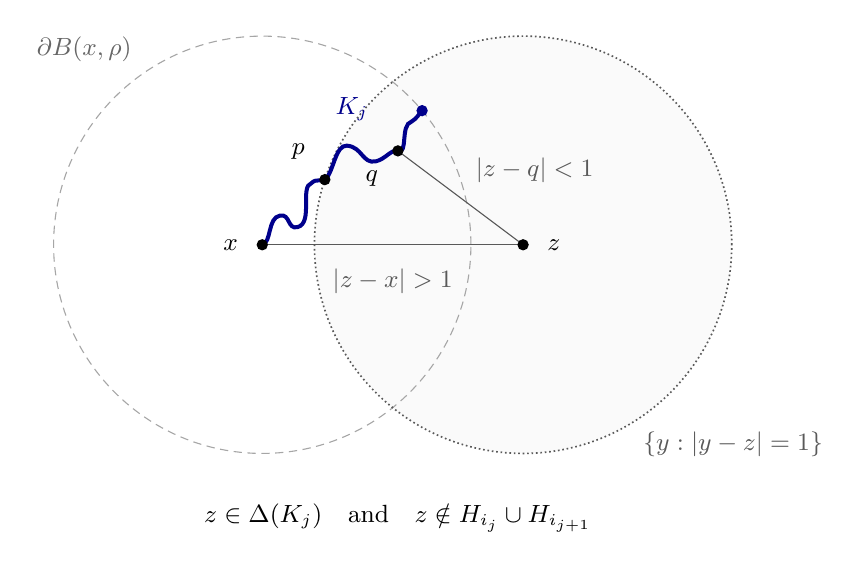
\begin{tikzpicture}[x=2.65cm,y=2.65cm,font=\small,
  point/.style={circle,fill=black,inner sep=1.45pt}]
  \coordinate (X) at (0,0);
  \coordinate (Z) at (1.25,0);
  \coordinate (Q) at (.65,.45);
  \coordinate (P) at (.3,{sqrt(1-.95*.95)});
  \coordinate (F) at ({cos(40)},{sin(40)});

  \fill[black!2] (Z) circle[radius=1];
  \draw[black!35,densely dashed] (X) circle[radius=1];
  \node[black!60,anchor=south east] at (-.58,.83)
    {$\partial B(x,\rho)$};
  \draw[black!65,densely dotted,semithick] (Z) circle[radius=1];
  \node[black!65,anchor=north west] at (1.78,-.85)
    {$\{y:|y-z|=1\}$};

  \draw[black!65] (X) -- node[below=5pt] {$|z-x|>1$} (Z);
  \draw[black!65] (Q) -- node[above right=2pt] {$|z-q|<1$} (Z);

  \draw[blue!55!black,line width=1.45pt,line cap=round]
    (X) .. controls (.045,.01) and (.025,.13) .. (.085,.14)
    .. controls (.135,.15) and (.12,.07) .. (.17,.085)
    .. controls (.245,.105) and (.18,.28) .. (.235,.295)
    .. controls (.26,.32) and (.28,.30) .. (P)
    .. controls (.34,.34) and (.35,.48) .. (.405,.475)
    .. controls (.48,.47) and (.48,.385) .. (.545,.40)
    .. controls (.59,.41) and (.62,.46) .. (Q)
    .. controls (.70,.43) and (.66,.575) .. (.715,.59)
    .. controls (.74,.605) and (.75,.625) .. (F);
  \node[blue!55!black,anchor=south] at (.43,.55) {$K_j$};

  \node[point,label={[label distance=3pt]left:$x$}] at (X) {};
  \node[point,label={[label distance=3pt]right:$z$}] at (Z) {};
  \node[point,label={[label distance=3pt]below left:$q$}] at (Q) {};
  \node[point,label={[label distance=3pt]above left:$p$}] at (P) {};
  \node[point,fill=blue!55!black] at (F) {};
  \node[align=center] at (.65,-1.31)
    {$z\in\Delta(K_j)$\quad and\quad
      $z\notin H_{i_j}\cup H_{i_{j+1}}$};
\end{tikzpicture}

\caption{The strict inequalities $|z-q|<1<|z-x|$, with $x,q\in K_j$,
put $z$ in $\Delta(K_j)$. Connectedness supplies a point $p\in K_j$
with $|z-p|=1$. Both endpoint essential supports are excluded from $\Delta(K_j)$. The shape is schematic: the proof assumes neither an arc nor
a smooth interface nor a tangent at $x$.}
\label{fig:exclusion-continuum}
\end{figure}

\subsection{Disk averages and missing edges}

We begin with continuous probability coordinates.  Their unit-distance
inequality will yield color exclusions from the straddling regions of
the limiting sets.  Small overlaps for missing transition edges will
control the disks removed from the approximation.

For $\epsilon>0$, set
\[
 p_i^\epsilon(q)=\frac1{\pi\epsilon^2}
                     \int_{B(0,\epsilon)}a_i(q+v)\,dv.
\]
These are continuous probability coordinates:
$p_i^\epsilon\ge0$ and $\sum_i p_i^\epsilon=1$ everywhere.
The symmetric-difference estimate for two disks gives
$\operatorname{Lip}(p_i^\epsilon)\le C/\epsilon$, with an absolute
constant $C$.  Approximation by local averages and Lebesgue
differentiation give $p_i^\epsilon\to a_i$ in $L^1_{\rm loc}$ and
almost everywhere as $\epsilon\downarrow0$.

\begin{lemma}[Disk inequalities and support detection]
\label{lem:transitions-disk-averages}
For every pair $q,z\in\R^2$ with $|q-z|=1$ and every label $i$,
\begin{equation}
 p_i^\epsilon(q)+p_i^\epsilon(z)\le1.
 \label{eq:source-17}
\end{equation}
If $q_n\to q$, $\epsilon_n\to0$, and
$\liminf_n p_i^{\epsilon_n}(q_n)>0$, then $q\in H_i$.
\end{lemma}

\begin{proof}
Translate $q$ and $z$ by the same vector uniformly distributed in
$B(0,\epsilon)$.  Almost every such translation puts both points in
the typical set.  They cannot then both have color $i$; averaging
proves \eqref{eq:source-17}.  Thus this inequality has no exceptional
unit pairs.  For the last assertion, every neighborhood of $q$
eventually contains $B(q_n,\epsilon_n)$, and the stated lower bound
makes its intersection with $A_i$ have positive area.
\end{proof}

\begin{lemma}[A missing edge has small overlap]
\label{lem:transitions-missing-edge}
If $ij\notin\Gamma_x$, there is a ball $B$ about $x$ such that, for
every smaller ball $B'$ with $\overline{B'}\subset B$,
\begin{equation}
 \int_{B'}p_i^\epsilon(q)p_j^\epsilon(q)\,dq=o(\epsilon).
 \label{eq:source-18}
\end{equation}
For any ball $B''$ with $\overline{B''}\subset B'$ and any fixed
$\alpha>0$, the set
\[
 \{q\in B'':p_i^\epsilon(q)>\alpha,\quad
                    p_j^\epsilon(q)>\alpha\}
\]
can be covered by finitely many open disks whose total radii tend to
zero as $\epsilon\downarrow0$.  Every point of the set lies in a disk
interior.
\end{lemma}

\begin{proof}
The negation of \eqref{eq:source-14}, and nonnegativity of $D_{ij}$,
give a ball $B$ with $D_{ij}(B,h)=o(|h|)$.  More explicitly, for all
sufficiently small $r>0$ put
\[
 \omega(r)=\sup_{0<|h|\le r}\frac{D_{ij}(B,h)}{|h|};
 \qquad \omega(r)\longrightarrow0.
\]
For independent uniform vectors $h_1,h_2\in B(0,\epsilon)$, expand the
product of the two disk averages and integrate over $q\in B'$.  When
$\epsilon<\dist(\overline{B'},\R^2\setminus B)$, the change of root
$r=q+h_1$ bounds the area where $c(q+h_1)=i$ and $c(q+h_2)=j$ by
\[
 D_{ij}(B,h_2-h_1)\le 2\epsilon\omega(2\epsilon).
\]
For $h_1=h_2$ the simultaneous event is empty.  Fubini now gives
\eqref{eq:source-18}, with a bound uniform over the two shifts.

Take a square grid with side $\ell=c_\alpha\epsilon$, where
$c_\alpha>0$ is fixed small enough that the Lipschitz oscillation of
either probability on a square is at most $\alpha/2$.  Select all
squares touching the displayed violation set in $B''$.  Their number
$N_\epsilon$ is finite, and for small $\epsilon$ each lies in $B'$ and
has both probabilities at least $\alpha/2$ throughout.  Disjointness
of their interiors and \eqref{eq:source-18} imply
\[
 N_\epsilon\ell^2\frac{\alpha^2}{4}=o(\epsilon),
 \qquad N_\epsilon\epsilon=o(1).
\]
Cover every selected closed square by the open disk with the same
center and radius $\ell$.  These disks strictly contain the squares
and have total radii $N_\epsilon\ell=o(1)$.
\end{proof}

\subsection{Graph-valued maps outside small core disks}

The preceding overlap bound allows us to remove all simultaneous
threshold violations associated with missing edges.  Fix
$0<\alpha<1/5$, and define
\begin{equation}
 q_i^\epsilon(z)=
 \frac{(p_i^\epsilon(z)-\alpha)_+}
      {\sum_{k\in\mathcal I}(p_k^\epsilon(z)-\alpha)_+},
 \qquad i\in\mathcal I.
 \label{eq:source-22}
\end{equation}
The denominator is positive because the five probabilities sum to one.
Thus $q^\epsilon$ is a continuous map into the simplex of probability
vectors on $\mathcal I$.  Let $\mathscr G$ be the one-skeleton of that
simplex, realized as the complete graph on its five vertices.  In
particular, $q_i^\epsilon(z)>0$ if and only if
$p_i^\epsilon(z)>\alpha$.

Choose a closed square $Q$ of side ten with
$\partial Q\cap\mathcal L=\varnothing$.  Such a square is obtained by
a small translation: local finiteness leaves only finitely many points
to avoid near the boundary of all squares in that translation family.
Choose a larger closed square $Q'$ containing $Q$ in its interior, and
write $L_0=\mathcal L\cap Q'$, a finite set by
Theorem~\ref{thm:cyclic-local-finiteness}.

\begin{lemma}[Small holes and tree fillings]
\label{lem:interfaces-hole-maps}
There are $\epsilon_n\downarrow0$ and finite families $\mathcal H_n$
of open disks with pairwise disjoint closures such that their total
radii tend to zero and the following hold for all sufficiently large
$n$.
\begin{enumerate}
\item For each $x\in L_0$, precisely one disk of $\mathcal H_n$ is
designated the core disk $B_{n,x}$ and contains $x$ in its interior.
Different points give different core disks.  If $x\in Q$, then
$\overline{B_{n,x}}\subset\operatorname{int}(Q)$; if $x\notin Q$, then
$\overline{B_{n,x}}\cap Q=\varnothing$.
\item The map $q^{\epsilon_n}$ takes values in $\mathscr G$ on
$Q\setminus\bigcup_{B\in\mathcal H_n}B$.
\item There is a continuous map
\begin{equation}
 g_n:Q\setminus\bigcup_{x\in L_0\cap Q}B_{n,x}
       \longrightarrow\mathscr G
 \label{eq:source-23}
\end{equation}
equal to $q^{\epsilon_n}$ outside all the open disks of
$\mathcal H_n$.  It is obtained by filling the non-core disks through
trees, preserving their boundary values.
\end{enumerate}
\end{lemma}

\begin{proof}
Fix a small $\delta>0$.  Start with the original core disks
$B(x,\delta)$, $x\in L_0$, and put
\[
 M_\delta=Q'\setminus\bigcup_{x\in L_0}B(x,\delta).
\]
This is compact, and every $\Gamma_z$, $z\in M_\delta$, is a forest,
including any isolated vertices.  For each nonedge of $\Gamma_z$,
Lemma~\ref{lem:transitions-missing-edge} supplies a ball on which the
corresponding simultaneous threshold violations admit finite open
disk covers with total radii tending to zero as $\epsilon\to0$.
There are finitely many nonedges, so choose one radius $s_z>0$
working for all of them.  More explicitly, choose it small enough
to have the transition estimate on $B(z,3s_z)$, the integral
estimate on $B(z,2s_z)$, and the disk covers for violations in
$B(z,s_z)$.  The covers include the violation points in the
interiors of their disks.

Choose finitely many balls $B(z,s_z)$ covering $M_\delta$, and let
$\lambda_\delta>0$ be a Lebesgue number of this cover on $M_\delta$.
For each selected ball, mark all the disks covering violations for
its forest's nonedges.  These additional disks form a finite family
whose total radii $m_{\delta,\epsilon}$ tend to zero for this fixed
$\delta$.  At a point of $M_\delta$ outside all marked disks, the
positive coordinates of \eqref{eq:source-22} form a clique in the
forest of every selected ball containing the point.  They therefore
number at most two, and a two-element set is a forest edge.  This
proves the required local graph-valued assertion.

We next merge disks until their closures are pairwise disjoint.
Whenever two current disks have intersecting closures, replace them
by an open disk strictly containing both closures, with radius at
most the sum of their radii plus a prescribed positive error.
An enclosing disk with radius at most the sum exists by choosing its
center on the line of centers; in the containment case the larger
disk suffices.  A slight enlargement makes containment strict.
Each merge reduces the finite number of disks, so the sum of all
enlargement errors can be made less than any specified
$\eta>0$, using the initial number as a bound on the number of merges.

A final disk is called core if its merger class contains an original
core disk.  Every final boundary avoids every original disk interior.
The total final radii are at most
\[
 |L_0|\delta+m_{\delta,\epsilon}+\eta,
\]
and each final non-core radius is at most
$m_{\delta,\epsilon}+\eta$.  Take $\delta_n\downarrow0$.
After fixing $\delta_n$, its finite cover, and its Lebesgue number,
choose $\epsilon_n$ and the merger errors so that
\[
 \epsilon_n<\min\{1/n,\epsilon_{n-1}/2\},\qquad
 m_{\delta_n,\epsilon_n}+\eta_n
   <\min\{1/n,\lambda_{\delta_n}/3\},
\]
omitting the preceding-$\epsilon$ condition at $n=1$.
The total final radii now tend to zero.

For large $n$, no final disk can contain two distinct points of $L_0$:
its diameter is smaller than their minimum positive separation.
Every original core disk belongs to some final disk, so this gives
exactly one core disk for each point.  Since a disk of radius $r$
containing $x$ lies in $B(x,2r)$, the positive distances between the
finitely many points of $L_0$ and $\partial Q$ give the asserted
positions of the core disks.

Consider a final non-core disk whose closure meets $Q$.  Its vanishing
diameter puts its entire closed disk inside $Q'$ for large $n$.
Moreover, its closure is disjoint from every final core closure,
and these final core disks contain all the original core disks.
It therefore lies outside all original core interiors, hence in
$M_{\delta_n}$.  Its diameter is less than $\lambda_{\delta_n}$,
so its entire closed disk lies in one selected forest ball.
Its boundary avoids all original marked interiors.  The original
map $q^{\epsilon_n}$ thus maps that boundary into the selected
forest, and its connected boundary image lies in one component
tree, possibly a single vertex.  A finite tree is contractible,
so the boundary map extends continuously over the closed disk
with values in that tree.  If the disk crosses $\partial Q$,
make the extension on the whole disk and restrict it to $Q$.

Outside all final open disks, every point of $Q$ belongs to
$M_{\delta_n}$ and avoids all original marked disks, so the original
map is graph-valued there.  Paste it to the finitely many tree
extensions.  Their closed disks have disjoint closures and agree
with the original map on their boundaries, so finite pasting proves
\eqref{eq:source-23}.  Empty disk lists require no operation.
\end{proof}

\subsection{A nontrivial core boundary}

We will repeatedly use the following area estimate.  For a closed
disk $\overline{B(u,r)}$ with $r<1$, every point at distance one from
some point of that disk belongs to
\[
 E(u,r)=\{z:1-r\le |z-u|\le1+r\}.
\]
The triangle inequality proves this containment, and the annulus
has area $4\pi r$.  For the families in
Lemma~\ref{lem:interfaces-hole-maps}, write
\begin{equation}
 E_n=\bigcup_{B(u,r)\in\mathcal H_n}E(u,r),
 \qquad
 |E_n|\le4\pi\sum_{B(u,r)\in\mathcal H_n}r\longrightarrow0.
 \label{eq:interfaces-annulus-area}
\end{equation}
Here all radii are less than one for large $n$.  If $z\notin E_n$,
no exact unit-distance point from $z$ lies in any closed hole disk,
regardless of how many disks there are.

\begin{lemma}[A cover obstruction on a square]
\label{lem:interfaces-cover}
A closed square of side ten has no relatively open cover of
multiplicity at most two and mesh at most two, where mesh is the
supremum of the Euclidean diameters of its members.
\end{lemma}

\begin{proof}
Compactness gives a finite subcover $U_1,\ldots,U_N$ with the same
bounds.  Choose $z_a\in U_a$.  There is a continuous partition of
unity $\phi_a$ with $\phi_a(z)>0$ only when $z\in U_a$; explicitly,
use $\dist(z,Q\setminus U_a)$ and normalize their sum.  None of the
$U_a$ equals $Q$, since its diameter would exceed two, so these
distance functions are well defined.  Set
\[
 F(z)=\sum_{a=1}^N\phi_a(z)z_a.
\]
Convexity gives $F(Q)\subset Q$.  At most two weights are positive
at any point, so the image is contained in the finite union of
segments $[z_a,z_b]$ and singleton vertices.  Also
\[
 |F(z)-z|
 \le\sum_a\phi_a(z)|z_a-z|\le2.
\]
For any $y\in Q$ with $\dist(y,\partial Q)>2$, the continuous map
$z\mapsto y+z-F(z)$ takes $Q$ into $Q$, since its image lies in
the closed radius-two disk about $y$.  The Brouwer fixed point
theorem, in its planar form
\citep[Theorem~1.9]{Hatcher2002}, therefore supplies a fixed point,
and at that point $F(z)=y$.  Thus $F(Q)$ contains the nonempty open
central region $\{y\in Q:\dist(y,\partial Q)>2\}$, impossible for a
finite union of segments.
\end{proof}

\begin{lemma}[Non-null core loops]
\label{lem:interfaces-core-loop}
For all sufficiently large $n$, some core disk $B_{n,x}$ contained
in $Q$ has a boundary loop whose image under $g_n$ is not null
homotopic in $\mathscr G$.
\end{lemma}

\begin{proof}
Otherwise, along an infinite subsequence all the core boundary
loops are null homotopic.  Extend each such loop over its disk
in $\mathscr G$, and paste to obtain a continuous map
$\widetilde g_n:Q\to\mathscr G$, still equal to $q^{\epsilon_n}$
outside all holes.  For each $i\in\mathcal I$, take the components
of the relatively open set
\[
 U_{n,i}=\{z\in Q:(\widetilde g_n(z))_i>0\}.
\]
The square and its relatively open subsets are locally path
connected; hence these components are open and path connected.
They form a cover of $Q$ of multiplicity at most two, since every
point of $\mathscr G$ has at most two positive coordinates.

We claim that the mesh of this component cover is at most $1+o(1)$.
If not, after restricting to a subsequence there are a fixed
constant $c>0$, a fixed label $i$, and paths in $U_{n,i}$ joining
points at distance greater than $1+c$.  Replace either endpoint
lying in a hole by a boundary point on the path.  The path must
exit that disk because the other endpoint is distant, and the
replacement changes the endpoint by at most the disk's diameter.
If both endpoints require replacement, their disks are distinct
for large $n$.  On every hole boundary the original map is
preserved.  Thus the replacement endpoints $a_n,b_n$ satisfy
\[
 p_i^{\epsilon_n}(a_n)>\alpha,\qquad
 p_i^{\epsilon_n}(b_n)>\alpha
\]
and remain at distance at least $1+c-o(1)$.  Pass to limits
$a_n\to a$, $b_n\to b$ in $Q$, with $|a-b|>1$.
Lemma~\ref{lem:transitions-disk-averages} gives $a\in H_i$.

Choose a sufficiently small fixed open plane ball $U$ about $a$.
For all large $n$ and every $z\in U$, the distances to $a_n$ and
$b_n$ are strictly below and strictly above one, respectively.
Continuity along the path supplies a point at exact distance one
from $z$.  If $z\notin E_n$, every such crossing point is outside
all closed hole disks by \eqref{eq:interfaces-annulus-area}.
At this point $\widetilde g_n=q^{\epsilon_n}$ and its $i$th
coordinate is positive, so $p_i^{\epsilon_n}>\alpha$.
The pointwise inequality \eqref{eq:source-17} therefore gives
$p_i^{\epsilon_n}(z)\le1-\alpha$.

It follows that
\begin{equation}
 \alpha |A_i\cap U|
 \le
 \norm{p_i^{\epsilon_n}-a_i}_{L^1(U)}
      +\alpha|E_n\cap U|
 \longrightarrow0.
 \label{eq:interfaces-mesh-measure}
\end{equation}
The convergence uses local $L^1$ convergence of disk averages and
\eqref{eq:interfaces-annulus-area}.  This contradicts $a\in H_i$,
which requires positive $A_i$-measure in $U$.  The mesh claim
follows.  For large $n$ the mesh is therefore at most two,
contradicting Lemma~\ref{lem:interfaces-cover}.  This argument also
rules out the possibility of having no core disks in $Q$.
\end{proof}

\subsection{Graph words and annular crossings}

We now have a graph-valued map with a non-null loop around a core disk.
To turn that loop into connected crossing sets, we identify edge
midpoints that every homotopic loop must meet.  We first recall the
reduced-path argument for graphs; compare
\citet[Section~1.A]{Hatcher2002}.

\begin{lemma}[Midpoint detection by a reduced circuit]
\label{lem:interfaces-graph-word}
Let $G$ be a finite connected simple graph.  Every nontrivial free
homotopy class of loops in $G$ has a nonempty cyclically reduced closed
edge word $W$.  Such a word contains a simple cycle.  Moreover, if $m$
is the midpoint of any edge occurring in $W$, every loop freely
homotopic to a nonzero power of $W$ meets $m$.
\end{lemma}

\begin{proof}
An edge path is reduced when consecutive edges never reverse each
other, and a reduced closed edge path is cyclically reduced when its
last and first edges do not reverse each other either.  Paths between
vertices, up to homotopy fixing their endpoints, have unique reduced
edge representatives.  One way to see this is to construct the covering
tree based at a vertex $v$: its vertices are reduced paths starting at
$v$, and its edges append one edge and then reduce.  Deleting the last
edge gives the unique path toward the empty word, so this covering
graph is a tree.  The map recording the endpoint is a bijection on
each incident-edge star and hence a covering map.  Lifting a path to
this tree and contracting it to the unique simple path between its
lifted endpoints proves existence and uniqueness of the reduced
representative.  These contractions apply to arbitrary continuous
paths: their compact images in the locally finite covering tree lie
in finite subtrees.

Move a loop's basepoint to a vertex along a path, reduce its edge
word, and successively trim inverse first and last edges.  The result
is cyclically reduced and is empty precisely when the loop is null
homotopic.  Moving the basepoint, or following the basepoint during a
free homotopy, changes the based class by conjugation.

We record how conjugation affects a nonempty cyclically reduced word.
First reduce the conjugating path $P$ in $PWP^{-1}$.  At the last edge
of $P$, cancellation against one end of $W$ shortens $P$ and moves
one edge of $W$ to its other end.  This only rotates $W$ cyclically.
Cancellation at both ends of $W$ at once is impossible because $W$
is cyclically reduced.  If there is no cancellation at either end,
the conjugating path is simply removed when the whole closed word is
cyclically trimmed.  Induction on the length of $P$ shows that
conjugation leaves the cyclically reduced circuit unchanged up to
cyclic rotation.

A nonzero power of $W$ is already cyclically reduced: concatenate
copies of $W$ for a positive power, or copies of its reversed inverse
for a negative power.  Its cyclic reduction therefore uses every edge
of $W$.  On the other hand, $G\setminus\{m\}$ deformation retracts onto
the graph with the edge containing $m$ deleted: contract its two
remaining half-open stubs to their endpoint vertices.  A loop avoiding
$m$ consequently has a reduced circuit using no such edge, and cannot
be freely homotopic to a nonzero power of $W$.

Finally, take a shortest nonempty subloop between repeated vertices
of $W$.  It has no repeated interior vertex.  Its length is not one,
since $G$ has no loop edges, and is not two, since that would be an
immediate reversal in a simple graph.  Thus it is a simple cycle.
\end{proof}

\begin{lemma}[A connected midpoint preimage crosses the annulus]
\label{lem:interfaces-annular-crossing}
Let $B$ be an open disk containing $x$, with
$\overline B\subset B(x,\rho)$, and set
$\mathcal A=\overline{B(x,\rho)}\setminus B$.
Suppose $g:\mathcal A\to G$ is continuous, where $G$ is a finite
connected simple graph, and the image of the counterclockwise inner
boundary has nonempty cyclically reduced word $W$.  If $m$ is the
midpoint of an edge occurring in $W$, then $g^{-1}(\{m\})$ has a
compact connected component meeting both boundary circles of
$\mathcal A$.
\end{lemma}

\begin{proof}
Every ray from $x$ meets $\partial B$ once, at a positive radius
$r(\theta)$ depending continuously on the angle.  Radial interpolation
between $r(\theta)$ and $\rho$ identifies $\mathcal A$ with a closed
annulus.  In particular, winding number about $x$ identifies its
fundamental group with $\Z$, with the counterclockwise inner boundary
as generator.

Put $Z=g^{-1}(\{m\})$.  This is a compact metric space.  Suppose no
component of $Z$ meets both boundaries, and write
$I=Z\cap\partial B$ and $O=Z\cap\partial B(x,\rho)$ for its compact
inner and outer contact sets.  We first obtain a disjoint compact partition
$Z=Z_1\sqcup Z_2$ with $I\subset Z_1$ and $O\subset Z_2$.

In any compact metric space, a point's component is the intersection
of all of its clopen neighborhoods.  Indeed, this intersection
contains the component.  If it were disconnected, its two nonempty
compact parts could be enclosed in disjoint open sets.  A finite
intersection of clopen neighborhoods already lies in their union,
by compactness of the complement of that union.  Intersecting this
clopen set with the open set containing the original point gives
a smaller clopen neighborhood omitting the other part, a
contradiction.  The intersection is therefore connected and equals
the component.

Thus, for each point of $I$ and each point of $O$, some clopen
neighborhood of the first omits the second.  Compactness of $O$
permits a finite intersection producing a clopen neighborhood of
the first point disjoint from all of $O$.  Compactness of $I$
then permits a finite union containing all of $I$ and still
disjoint from $O$.  Take this union as $Z_1$ and its complement in
$Z$ as $Z_2$.  If either $I$ or $O$ is empty, use $Z_1=\varnothing$
or $Z_1=Z$, respectively.  This proves the partition assertion.

The set
\[
 C_1=Z_1\cup\overline B
\]
is compact, lies in the open outer disk, and is disjoint from $Z_2$.
Choose a sufficiently fine translated square grid, with $x$ on no
grid line, and take every closed grid cell meeting $C_1$.  Their
finite union $V$ lies in the open outer disk and avoids $Z_2$, by the
positive compact separations.  Also $C_1\subset\operatorname{int}(V)$:
at a point of $C_1$ on a grid edge or vertex, all adjacent cells
are included.  Consequently $\partial V$ lies in $\mathcal A$
and avoids $Z_1\cup Z_2=Z$.

Orient each selected square boundary counterclockwise and cancel
shared edges.  The remaining edges lie on $\partial V$ and form
a balanced finite directed chain, so they decompose into closed
polygonal loops.  Their total winding about $x$ is one.  Indeed,
winding is additive before and after cancellation, and exactly one
selected square contains $x$ in its interior; its winding is one
and that of every other selected square is zero.  At least one
of the resulting loops has nonzero winding, say $d$.  Its image
under $g$ avoids $m$, but the annulus calculation makes that image
freely homotopic to $W^d$.  This contradicts
Lemma~\ref{lem:interfaces-graph-word}.
\end{proof}

\subsection{Limiting continua and simultaneous color exclusions}

\begin{proof}[Proof of Proposition~\ref{prop:interface-cycle}]
Use the maps of Lemma~\ref{lem:interfaces-hole-maps} and the
non-null loops from Lemma~\ref{lem:interfaces-core-loop}.
Since $L_0\cap Q$ is finite, pass to a subsequence with a fixed
$x\in L_0\cap\operatorname{int}(Q)$ whose core boundary loop
is non-null at every index.  Choose $\rho>0$ so small that
$\overline{B(x,\rho)}\subset\operatorname{int}(Q)$ and contains no
other point of $L_0$.  Decreasing $\rho$ if necessary, the other
core closed disks are disjoint from $\overline{B(x,\rho)}$ for
large $n$, while
$\overline{B_{n,x}}\subset B(x,\rho)$.  The map $g_n$ is therefore
defined on the closed annulus
\[
 \mathcal A_n=\overline{B(x,\rho)}\setminus B_{n,x}.
\]
The inner disk contains $x$ strictly; its possibly eccentric
position causes no difficulty for the radial annulus coordinates
used in Lemma~\ref{lem:interfaces-annular-crossing}.

Let $W_n$ be a nonempty cyclically reduced circuit representing the
image of the counterclockwise inner boundary.  By
Lemma~\ref{lem:interfaces-graph-word}, it contains a simple cycle.
There are only finitely many simple cycles in the complete graph
on five vertices.  Pass to a subsequence with one chosen cycle,
of length $\ell\in\{3,4,5\}$, and label its vertices
$i_0,\ldots,i_{\ell-1}$ in cyclic order.  For each of its edge
midpoints $m_j$, Lemma~\ref{lem:interfaces-annular-crossing} gives
a compact connected component
\[
 K_{n,j}\subset g_n^{-1}(\{m_j\})\cap\mathcal A_n
\]
meeting both annulus boundaries.

Take Hausdorff limits along a common further subsequence for the
finitely many indices $j$:
\[
 K_{n,j}\longrightarrow K_j\subset\overline{B(x,\rho)}.
\]
The nonempty compact subsets of a compact metric space are compact
in the Hausdorff metric.  For completeness, finite nets give total
boundedness of this hyperspace, and for a Hausdorff-Cauchy sequence
the set of limits of convergent point selections is its nonempty
compact Hausdorff limit, proving completeness.  Connectedness also
passes to the limit: a disconnection of $K_j$ into two nonempty
compact parts gives disjoint separated neighborhoods containing
every sufficiently close $K_{n,j}$, with each neighborhood met,
contradicting connectedness of $K_{n,j}$.

Each $K_{n,j}$ meets $\partial B_{n,x}$.  These contact points tend
to $x$, because the disk contains $x$ and its diameter tends to
zero.  Hence $x\in K_j$.  Outer-boundary contact and compactness
likewise give $K_j\cap\partial B(x,\rho)\ne\varnothing$.
In particular each $K_j$ is nontrivial.

We prove the support exclusion for either endpoint
$i\in\{i_j,i_{j+1}\}$.  At a point of $K_{n,j}$ outside all holes,
$g_n=q^{\epsilon_n}$ has value $m_j$, whose two endpoint
coordinates are $1/2$.  Formula~\eqref{eq:source-22} therefore gives
$p_i^{\epsilon_n}>\alpha$ there.

Fix any closed ball $U$ of positive radius contained in
$\Delta(K_j)$.  The strict inequalities defining the straddling
region hold with a positive uniform margin on $U$.  For every
$z$, either distance extremum changes by at most
$d_{\rm H}(K_{n,j},K_j)$ when $K_j$ is replaced by $K_{n,j}$.
Thus, for all sufficiently large $n$, the distances from every
$z\in U$ to points of $K_{n,j}$ straddle one.  The continuous
image of the connected set $K_{n,j}$ under $q\mapsto|z-q|$
is an interval, so some point of $K_{n,j}$ is at exact distance
one from $z$.

For $z\in U\setminus E_n$, that point is outside every closed hole
disk.  The preceding endpoint probability bound and
\eqref{eq:source-17} give $p_i^{\epsilon_n}(z)\le1-\alpha$.
Exactly as in \eqref{eq:interfaces-mesh-measure},
\[
 \alpha |A_i\cap U|
 \le \norm{p_i^{\epsilon_n}-a_i}_{L^1(U)}
       +\alpha |E_n\cap U|\longrightarrow0.
\]
Thus $A_i$ has zero measure in $U$.  Every point of the open set
$\Delta(K_j)$ lies in the interior of such a ball, and consequently
has a neighborhood of zero $A_i$-measure.  By the definition of
$H_i$, this proves $H_i\cap\Delta(K_j)=\varnothing$ for both
endpoint labels.

Finally, connectedness and the two contact conditions imply
\[
 \{|q-x|:q\in K_j\}=[0,\rho].
\]
Choose points in $K_j$ at radii $\rho/k$, $k\ge2$, and pass to a
subsequence of their unit directions converging to some $v_j\in S$.
Relabel these points as $q_{j,k}$.  They supply the required
sequences and complete the proof.
\end{proof}
